\documentclass{article}\usepackage[]{graphicx}\usepackage[]{color}
%% maxwidth is the original width if it is less than linewidth
%% otherwise use linewidth (to make sure the graphics do not exceed the margin)
\makeatletter
\def\maxwidth{ %
  \ifdim\Gin@nat@width>\linewidth
    \linewidth
  \else
    \Gin@nat@width
  \fi
}
\makeatother

\definecolor{fgcolor}{rgb}{0.345, 0.345, 0.345}
\newcommand{\hlnum}[1]{\textcolor[rgb]{0.686,0.059,0.569}{#1}}%
\newcommand{\hlstr}[1]{\textcolor[rgb]{0.192,0.494,0.8}{#1}}%
\newcommand{\hlcom}[1]{\textcolor[rgb]{0.678,0.584,0.686}{\textit{#1}}}%
\newcommand{\hlopt}[1]{\textcolor[rgb]{0,0,0}{#1}}%
\newcommand{\hlstd}[1]{\textcolor[rgb]{0.345,0.345,0.345}{#1}}%
\newcommand{\hlkwa}[1]{\textcolor[rgb]{0.161,0.373,0.58}{\textbf{#1}}}%
\newcommand{\hlkwb}[1]{\textcolor[rgb]{0.69,0.353,0.396}{#1}}%
\newcommand{\hlkwc}[1]{\textcolor[rgb]{0.333,0.667,0.333}{#1}}%
\newcommand{\hlkwd}[1]{\textcolor[rgb]{0.737,0.353,0.396}{\textbf{#1}}}%

\usepackage{framed}
\makeatletter
\newenvironment{kframe}{%
 \def\at@end@of@kframe{}%
 \ifinner\ifhmode%
  \def\at@end@of@kframe{\end{minipage}}%
  \begin{minipage}{\columnwidth}%
 \fi\fi%
 \def\FrameCommand##1{\hskip\@totalleftmargin \hskip-\fboxsep
 \colorbox{shadecolor}{##1}\hskip-\fboxsep
     % There is no \\@totalrightmargin, so:
     \hskip-\linewidth \hskip-\@totalleftmargin \hskip\columnwidth}%
 \MakeFramed {\advance\hsize-\width
   \@totalleftmargin\z@ \linewidth\hsize
   \@setminipage}}%
 {\par\unskip\endMakeFramed%
 \at@end@of@kframe}
\makeatother

\definecolor{shadecolor}{rgb}{.97, .97, .97}
\definecolor{messagecolor}{rgb}{0, 0, 0}
\definecolor{warningcolor}{rgb}{1, 0, 1}
\definecolor{errorcolor}{rgb}{1, 0, 0}
\newenvironment{knitrout}{}{} % an empty environment to be redefined in TeX

\usepackage{alltt}
\usepackage{enumerate}
\usepackage{amsmath}
\IfFileExists{upquote.sty}{\usepackage{upquote}}{}
\begin{document}

\title{\huge \textbf{Stat 207 HW4} \\}
\author{\large Cheng Luo 912466499 \\ \large Fan Wu 912538518}
\maketitle

\newpage
\mbox{}
\newpage

\section{27.6}

\begin{enumerate}[(a)]

\item

\begin{knitrout}
\definecolor{shadecolor}{rgb}{0.969, 0.969, 0.969}\color{fgcolor}\begin{kframe}
\begin{alltt}
  \hlstd{dat} \hlkwb{=} \hlkwd{read.table}\hlstd{(}\hlstr{"CH27PR06.txt"}\hlstd{)}
  \hlkwd{names}\hlstd{(dat)} \hlkwb{=} \hlkwd{c}\hlstd{(}\hlstr{"Y"}\hlstd{,} \hlstr{"S"}\hlstd{,} \hlstr{"A"}\hlstd{)}
  \hlstd{dat1} \hlkwb{=} \hlstd{dat}
  \hlstd{dat}\hlopt{$}\hlstd{A} \hlkwb{=} \hlkwd{factor}\hlstd{(dat}\hlopt{$}\hlstd{A)}
  \hlstd{dat}\hlopt{$}\hlstd{S} \hlkwb{=} \hlkwd{factor}\hlstd{(dat}\hlopt{$}\hlstd{S)}
  \hlstd{r} \hlkwb{=} \hlkwd{length}\hlstd{(}\hlkwd{unique}\hlstd{(dat}\hlopt{$}\hlstd{S))}
  \hlstd{a} \hlkwb{=} \hlkwd{length}\hlstd{(}\hlkwd{unique}\hlstd{(dat}\hlopt{$}\hlstd{A))}
  \hlstd{model} \hlkwb{=} \hlkwd{aov}\hlstd{(Y}\hlopt{~} \hlstd{A} \hlopt{+} \hlstd{S,} \hlkwc{data} \hlstd{= dat)}
  \hlstd{res} \hlkwb{=} \hlkwd{resid}\hlstd{(model)}
  \hlstd{res}
\end{alltt}
\begin{verbatim}
##           1           2           3           4           5           6 
## -1.27916667 -0.24166667  1.52083333 -0.84583333  0.69166667  0.15416667 
##           7           8           9          10          11          12 
##  0.62083333  0.05833333 -0.67916667  0.55416667  0.19166667 -0.74583333 
##          13          14          15          16          17          18 
##  0.52083333 -0.34166667 -0.17916667 -0.14583333  0.39166667 -0.24583333 
##          19          20          21          22          23          24 
##  0.98750000 -0.77500000 -0.21250000 -0.41250000  0.02500000  0.38750000
\end{verbatim}
\begin{alltt}
  \hlkwd{par}\hlstd{(}\hlkwc{mfrow} \hlstd{=} \hlkwd{c}\hlstd{(}\hlnum{1}\hlstd{,}\hlnum{2}\hlstd{))}
  \hlkwd{plot}\hlstd{(model,} \hlkwc{which} \hlstd{=} \hlnum{1}\hlstd{)}
  \hlkwd{plot}\hlstd{(model,} \hlkwc{which} \hlstd{=} \hlnum{2}\hlstd{)}
\end{alltt}
\end{kframe}
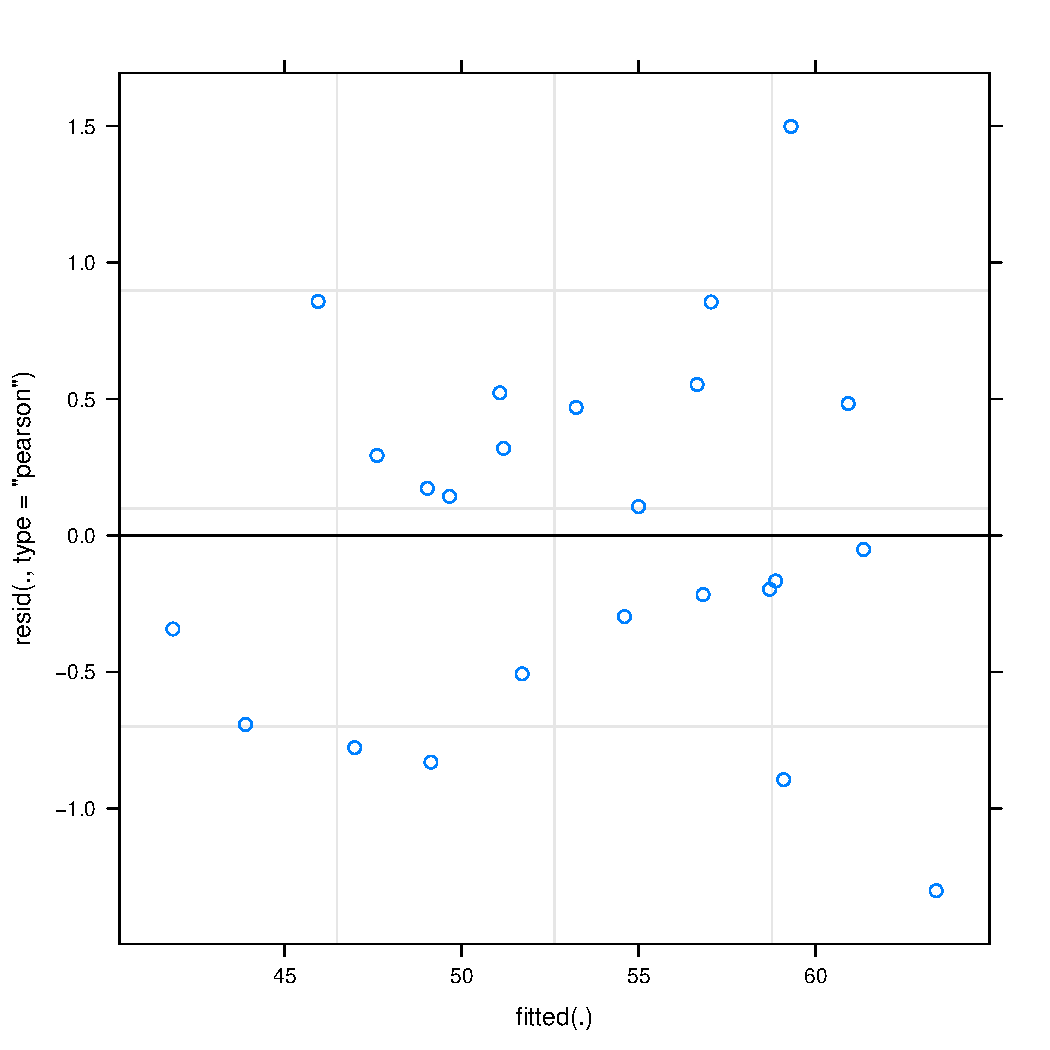
\includegraphics[width=\maxwidth]{figure/unnamed-chunk-1-1} 

\end{knitrout}

\qquad The residuals versus fitted values plots shows no sign for unequal variance.And the QQ-plot indicates approximately normal distribution, so that normality assumption seems to be reasonable, we can use repeated measures model here.

\item

\begin{knitrout}
\definecolor{shadecolor}{rgb}{0.969, 0.969, 0.969}\color{fgcolor}\begin{kframe}
\begin{alltt}
  \hlkwd{stripchart}\hlstd{(res} \hlopt{~} \hlstd{dat}\hlopt{$}\hlstd{A,} \hlkwc{method} \hlstd{=} \hlstr{'stack'}\hlstd{)}
\end{alltt}
\end{kframe}
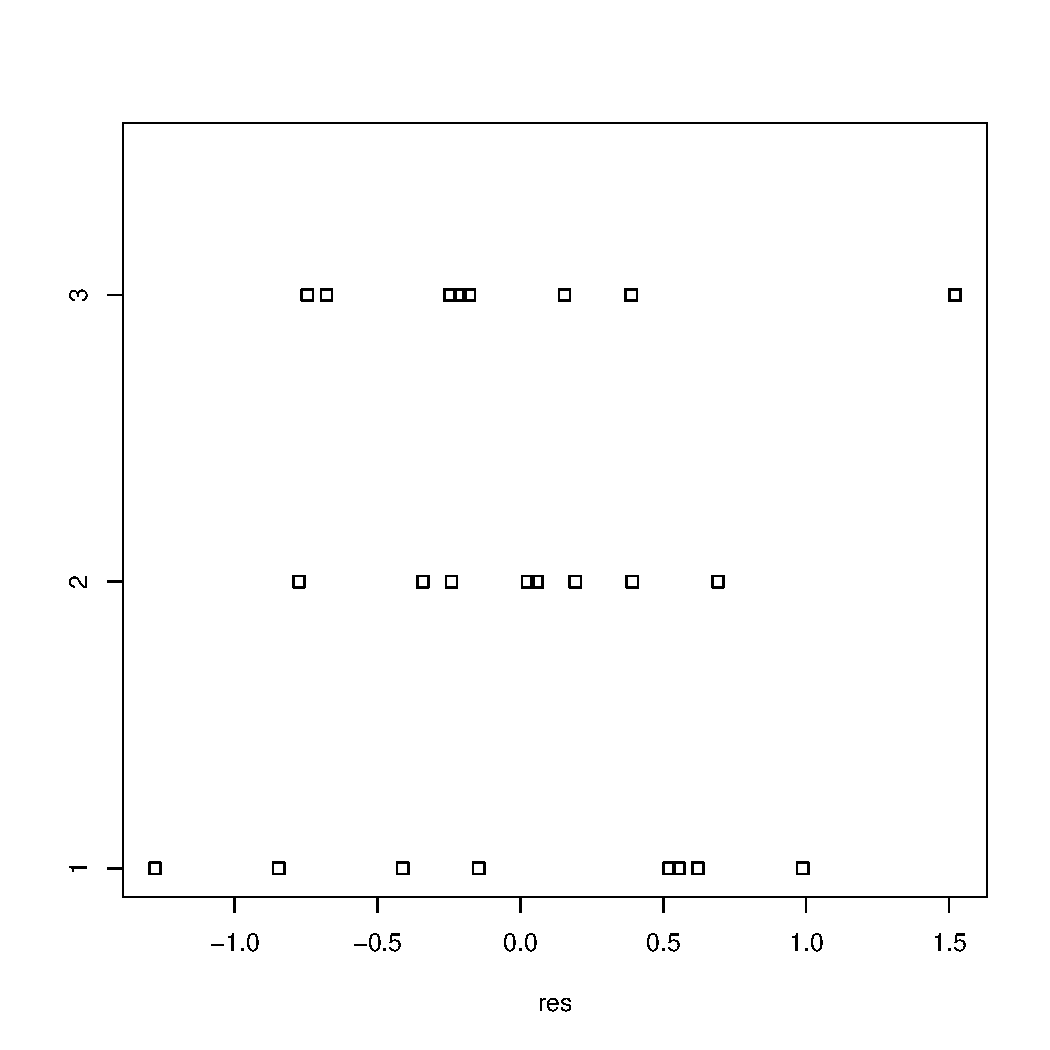
\includegraphics[width=\maxwidth]{figure/unnamed-chunk-2-1} 

\end{knitrout}

\qquad These plots do not indicate any correlations of the error terms within a price level, and thus suggest that no interference effects are present.

\item

\begin{knitrout}
\definecolor{shadecolor}{rgb}{0.969, 0.969, 0.969}\color{fgcolor}\begin{kframe}
\begin{alltt}
  \hlkwd{interaction.plot}\hlstd{(dat}\hlopt{$}\hlstd{A, dat}\hlopt{$}\hlstd{S, dat}\hlopt{$}\hlstd{Y)}
\end{alltt}
\end{kframe}
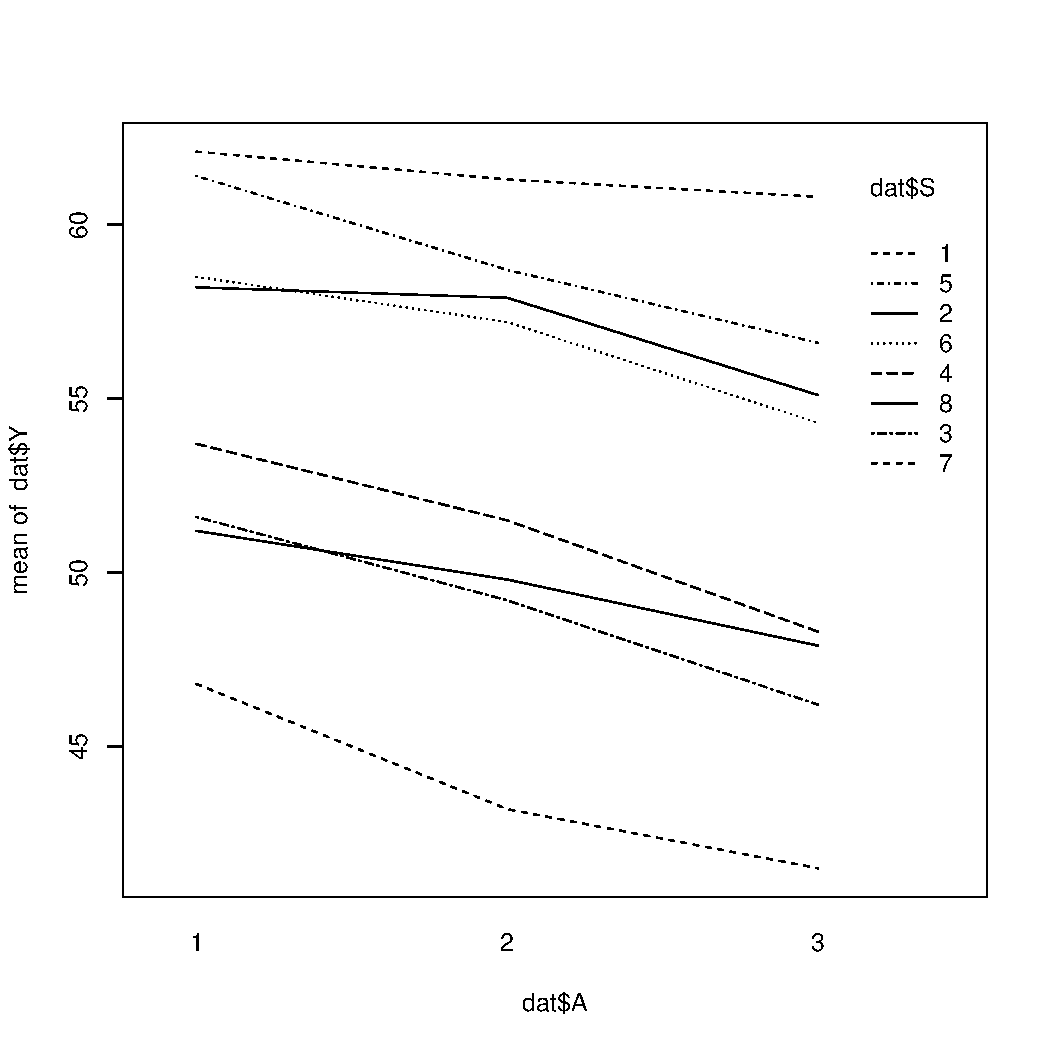
\includegraphics[width=\maxwidth]{figure/unnamed-chunk-3-1} 

\end{knitrout}

\qquad We see that the rating curves for the stores do not appear to exhibit substantial departures from being parallel, hence, the assumption of no interactions appear to be reasonable.

\item

\begin{knitrout}
\definecolor{shadecolor}{rgb}{0.969, 0.969, 0.969}\color{fgcolor}\begin{kframe}
\begin{alltt}
  \hlstd{ab} \hlkwb{=} \hlstd{dat1}\hlopt{$}\hlstd{S}\hlopt{*}\hlstd{dat1}\hlopt{$}\hlstd{A}
  \hlstd{model1} \hlkwb{=} \hlkwd{aov}\hlstd{(Y}\hlopt{~}\hlkwd{factor}\hlstd{(A)}\hlopt{+}\hlkwd{factor}\hlstd{(S)}\hlopt{+}\hlstd{ab,} \hlkwc{data} \hlstd{= dat1)}
  \hlkwd{anova}\hlstd{(model1)}
\end{alltt}
\begin{verbatim}
## Analysis of Variance Table
## 
## Response: Y
##           Df Sum Sq Mean Sq  F value    Pr(>F)    
## factor(A)  2  67.48  33.740  52.9429 5.653e-07 ***
## factor(S)  7 745.19 106.455 167.0410 1.056e-11 ***
## ab         1   1.29   1.288   2.0204    0.1787    
## Residuals 13   8.28   0.637                       
## ---
## Signif. codes:  0 '***' 0.001 '**' 0.01 '*' 0.05 '.' 0.1 ' ' 1
\end{verbatim}
\begin{alltt}
  \hlkwd{qf}\hlstd{(}\hlnum{1}\hlopt{-}\hlnum{0.01}\hlstd{,} \hlnum{1}\hlstd{,} \hlnum{13}\hlstd{)}
\end{alltt}
\begin{verbatim}
## [1] 9.073806
\end{verbatim}
\begin{alltt}
  \hlkwd{pf}\hlstd{(}\hlnum{2.0204}\hlstd{,} \hlnum{1}\hlstd{,} \hlnum{13}\hlstd{,} \hlkwc{lower.tail} \hlstd{=} \hlnum{FALSE}\hlstd{)}
\end{alltt}
\begin{verbatim}
## [1] 0.1787417
\end{verbatim}
\end{kframe}
\end{knitrout}

\begin{center}
$H_0$:$D = 0$

VS. $H_1$:$D \ne 0$

$F^*=\frac{SSAB^*/1}{SSrem*/(13)} = 1.288/0.637  =2.0204$

we can reject $H_0$ if $F^* > F(1-0.01;1,13)=9.073806$,otherwise reject$H_1$

so that reject $H_1$ because $F^*<9.073806$,

therefore, our conclusion implies that D equals zero, so there's no interactions, and P-value is 0.1787417.
\end{center}

\end{enumerate}

\section{27.7}

\begin{enumerate}[(a)]

\item

\begin{knitrout}
\definecolor{shadecolor}{rgb}{0.969, 0.969, 0.969}\color{fgcolor}\begin{kframe}
\begin{alltt}
  \hlstd{model} \hlkwb{=} \hlkwd{aov}\hlstd{(Y}\hlopt{~} \hlstd{A} \hlopt{+} \hlkwd{Error}\hlstd{(S}\hlopt{/}\hlstd{A),} \hlkwc{data} \hlstd{= dat)}
  \hlkwd{summary}\hlstd{(model)}
\end{alltt}
\begin{verbatim}
## 
## Error: S
##           Df Sum Sq Mean Sq F value Pr(>F)
## Residuals  7  745.2   106.5               
## 
## Error: S:A
##           Df Sum Sq Mean Sq F value   Pr(>F)    
## A          2  67.48   33.74   49.35 4.57e-07 ***
## Residuals 14   9.57    0.68                     
## ---
## Signif. codes:  0 '***' 0.001 '**' 0.01 '*' 0.05 '.' 0.1 ' ' 1
\end{verbatim}
\end{kframe}
\end{knitrout}

\item

\begin{knitrout}
\definecolor{shadecolor}{rgb}{0.969, 0.969, 0.969}\color{fgcolor}\begin{kframe}
\begin{alltt}
  \hlkwd{qf}\hlstd{(}\hlnum{1}\hlopt{-}\hlnum{0.05}\hlstd{,} \hlnum{2}\hlstd{,} \hlnum{14}\hlstd{)}
\end{alltt}
\begin{verbatim}
## [1] 3.738892
\end{verbatim}
\begin{alltt}
  \hlkwd{pf}\hlstd{(}\hlnum{49.35}\hlstd{,} \hlnum{2}\hlstd{,} \hlnum{14}\hlstd{,} \hlkwc{lower.tail} \hlstd{=} \hlnum{FALSE}\hlstd{)}
\end{alltt}
\begin{verbatim}
## [1] 4.564874e-07
\end{verbatim}
\end{kframe}
\end{knitrout}

\begin{center}
$H_0$:all $\tau_j$ equal zero(j=1,2,3)

VS. $H_1$:not all $\tau_j$ equal zero

$F^*=\frac{MSA}{MSE} = 33.74/0.68   = 49.35$

we can reject $H_0$ if $F^* > F(1-0.05;2,14)=3.738892$,otherwise reject$H_1$

so that reject $H_0$ because $F^*>3.738892$,

therefore, the mean sales of grapefruits differ for three price levels, and the P-value is 4.57e-07
\end{center}

\item

\begin{knitrout}
\definecolor{shadecolor}{rgb}{0.969, 0.969, 0.969}\color{fgcolor}\begin{kframe}
\begin{alltt}
  \hlstd{means} \hlkwb{=} \hlkwd{with}\hlstd{(dat,} \hlkwd{by}\hlstd{(Y, A, mean))}
  \hlstd{D1} \hlkwb{=} \hlstd{means[}\hlnum{1}\hlstd{]} \hlopt{-} \hlstd{means[}\hlnum{2}\hlstd{]}
  \hlstd{D2} \hlkwb{=} \hlstd{means[}\hlnum{1}\hlstd{]} \hlopt{-} \hlstd{means[}\hlnum{3}\hlstd{]}
  \hlstd{D3} \hlkwb{=} \hlstd{means[}\hlnum{2}\hlstd{]} \hlopt{-} \hlstd{means[}\hlnum{3}\hlstd{]}
  \hlstd{tukey} \hlkwb{=} \hlnum{1}\hlopt{/}\hlkwd{sqrt}\hlstd{(}\hlnum{2}\hlstd{)}\hlopt{*}\hlkwd{qtukey}\hlstd{(}\hlnum{0.95}\hlstd{, a, (a}\hlopt{-}\hlnum{1}\hlstd{)}\hlopt{*}\hlstd{(r}\hlopt{-}\hlnum{1}\hlstd{))}
  \hlstd{tukey}
\end{alltt}
\begin{verbatim}
## [1] 2.61728
\end{verbatim}
\begin{alltt}
  \hlstd{mstr.s} \hlkwb{=} \hlnum{0.68}
  \hlstd{s} \hlkwb{=} \hlkwd{sqrt}\hlstd{(}\hlnum{2}\hlopt{*}\hlstd{mstr.s}\hlopt{/}\hlstd{(r))}
  \hlstd{s}
\end{alltt}
\begin{verbatim}
## [1] 0.4123106
\end{verbatim}
\begin{alltt}
  \hlkwd{c}\hlstd{(D1}\hlopt{-}\hlstd{s}\hlopt{*}\hlstd{tukey, D1}\hlopt{+}\hlstd{s}\hlopt{*}\hlstd{tukey)}
\end{alltt}
\begin{verbatim}
##         1         1 
## 0.7583676 2.9166324
\end{verbatim}
\begin{alltt}
  \hlkwd{c}\hlstd{(D2}\hlopt{-}\hlstd{s}\hlopt{*}\hlstd{tukey, D2}\hlopt{+}\hlstd{s}\hlopt{*}\hlstd{tukey)}
\end{alltt}
\begin{verbatim}
##        1        1 
## 3.020868 5.179132
\end{verbatim}
\begin{alltt}
  \hlkwd{c}\hlstd{(D3}\hlopt{-}\hlstd{s}\hlopt{*}\hlstd{tukey, D3}\hlopt{+}\hlstd{s}\hlopt{*}\hlstd{tukey)}
\end{alltt}
\begin{verbatim}
##        2        2 
## 1.183368 3.341632
\end{verbatim}
\begin{alltt}
  \hlkwd{plot}\hlstd{(}\hlkwd{c}\hlstd{(}\hlopt{-}\hlnum{1}\hlstd{,} \hlnum{6}\hlstd{),} \hlkwd{c}\hlstd{(}\hlnum{0}\hlstd{,} \hlnum{0}\hlstd{),} \hlkwc{type} \hlstd{=} \hlstr{"l"}\hlstd{)}
  \hlkwd{points}\hlstd{(}\hlkwd{c}\hlstd{(D1}\hlopt{-}\hlstd{s}\hlopt{*}\hlstd{tukey, D1}\hlopt{+}\hlstd{s}\hlopt{*}\hlstd{tukey),} \hlkwd{c}\hlstd{(}\hlnum{0}\hlstd{,} \hlnum{0}\hlstd{),} \hlkwc{pch} \hlstd{=} \hlnum{1}\hlstd{)}
  \hlkwd{points}\hlstd{(}\hlkwd{c}\hlstd{(D2}\hlopt{-}\hlstd{s}\hlopt{*}\hlstd{tukey, D2}\hlopt{+}\hlstd{s}\hlopt{*}\hlstd{tukey),} \hlkwd{c}\hlstd{(}\hlnum{0}\hlstd{,} \hlnum{0}\hlstd{),} \hlkwc{pch} \hlstd{=} \hlnum{2}\hlstd{)}
  \hlkwd{points}\hlstd{(}\hlkwd{c}\hlstd{(D3}\hlopt{-}\hlstd{s}\hlopt{*}\hlstd{tukey, D3}\hlopt{+}\hlstd{s}\hlopt{*}\hlstd{tukey),} \hlkwd{c}\hlstd{(}\hlnum{0}\hlstd{,} \hlnum{0}\hlstd{),} \hlkwc{pch} \hlstd{=} \hlnum{3}\hlstd{)}
\end{alltt}
\end{kframe}
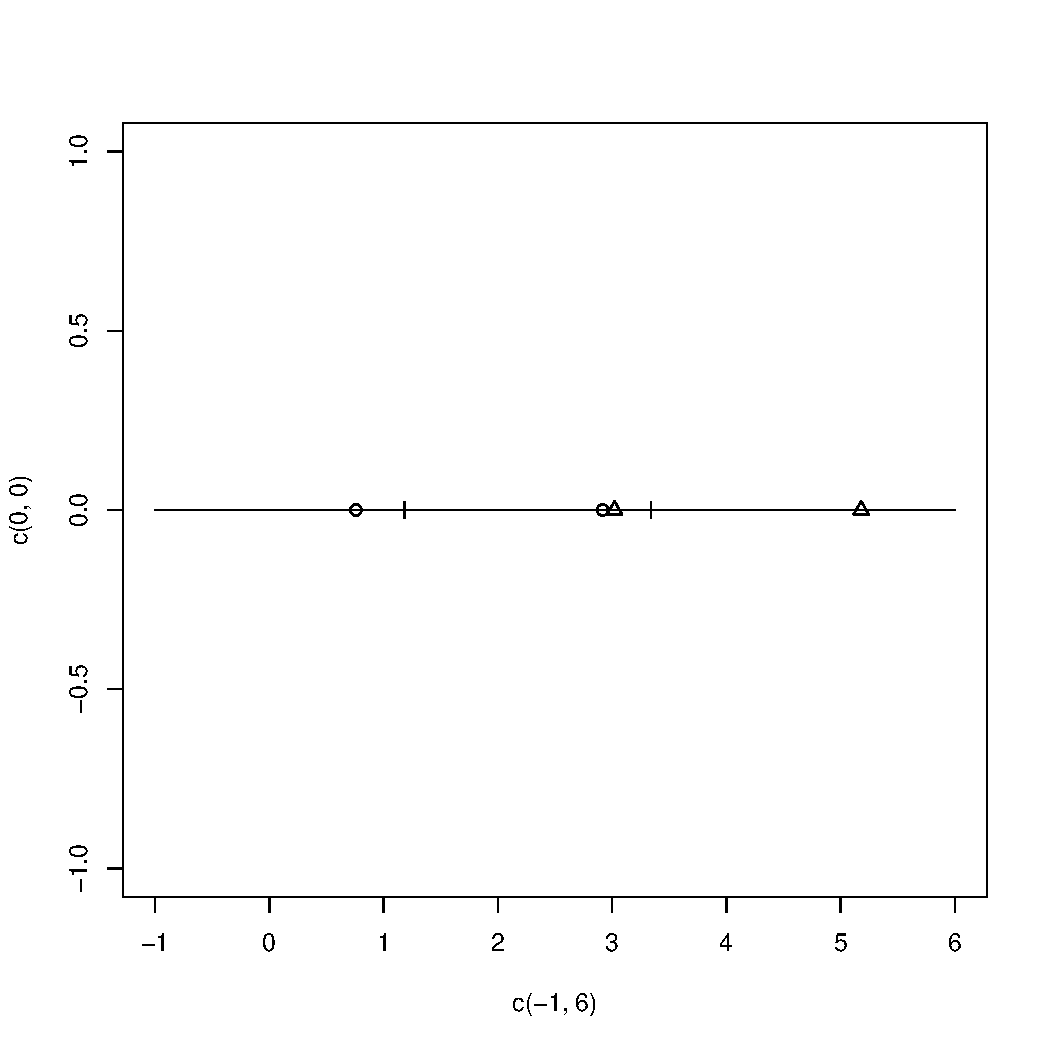
\includegraphics[width=\maxwidth]{figure/unnamed-chunk-7-1} 

\end{knitrout}

\begin{displaymath}
\begin{split}
\bar{Y}_{1\cdot \cdot} = 55.4375 &, \bar{Y}_{2\cdot \cdot} = 53.6 , \bar{Y}_{3\cdot \cdot} = 51.3375 \\
\hat{D}_1 = \bar{Y}_{1\cdot \cdot}-\bar{Y}_{2\cdot \cdot} = 1.8375 &,  \hat{D}_2 = \bar{Y}_{1\cdot \cdot}-\bar{Y}_{3\cdot \cdot}=4.1  , \hat{D}_3 = \bar{Y}_{2\cdot \cdot}-\bar{Y}_{3\cdot \cdot}=2.2625  \\
\text{Because we estimate all pairwise }& \text{comparisons, so we use tukey procedure}\\
S = \sqrt{\frac{MSTR.S}{r}*2} = 0.4123106 &, Tukey = \frac{1}{\sqrt{2}}\text{qtukey}(1-alpha, a, (a-1)*(r-1))=2.61728\\
\text{base on } &\hat{D}_i \pm S*Tukey\\
0.7583676 & \leq D_1 \leq 2.9166324  \\
3.020868 &\leq D_2 \leq 5.179132  \\
1.183368 &\leq D_3 \leq 3.341632   \\
\end{split}
\end{displaymath}

\item

\begin{displaymath}
\begin{split}
\hat{E} &= \frac{S_r^2}{MSTR.S} \\
        &= \frac{(s-1)MSS+s(r-1)*MSTR.S}{(sr-1)*MSTR.S}\\
        &= 48.36189
\end{split}
\end{displaymath}

\end{enumerate}

\section{27.18}

\begin{enumerate}[(a)]

\item

\begin{knitrout}
\definecolor{shadecolor}{rgb}{0.969, 0.969, 0.969}\color{fgcolor}\begin{kframe}
\begin{alltt}
  \hlstd{dat} \hlkwb{=} \hlkwd{read.table}\hlstd{(}\hlstr{"CH27PR18.txt"}\hlstd{)}
  \hlkwd{names}\hlstd{(dat)} \hlkwb{=} \hlkwd{c}\hlstd{(}\hlstr{"Y"}\hlstd{,} \hlstr{"S"}\hlstd{,} \hlstr{"A"}\hlstd{,} \hlstr{"B"}\hlstd{)}
  \hlstd{dat}\hlopt{$}\hlstd{S} \hlkwb{=} \hlkwd{factor}\hlstd{(dat}\hlopt{$}\hlstd{S)}
  \hlstd{dat}\hlopt{$}\hlstd{A} \hlkwb{=} \hlkwd{factor}\hlstd{(dat}\hlopt{$}\hlstd{A)}
  \hlstd{dat}\hlopt{$}\hlstd{B} \hlkwb{=} \hlkwd{factor}\hlstd{(dat}\hlopt{$}\hlstd{B)}
  \hlstd{s} \hlkwb{=} \hlkwd{length}\hlstd{(}\hlkwd{unique}\hlstd{(dat}\hlopt{$}\hlstd{S))}
  \hlstd{a} \hlkwb{=} \hlkwd{length}\hlstd{(}\hlkwd{unique}\hlstd{(dat}\hlopt{$}\hlstd{A))}
  \hlstd{b} \hlkwb{=} \hlkwd{length}\hlstd{(}\hlkwd{unique}\hlstd{(dat}\hlopt{$}\hlstd{B))}
  \hlstd{model} \hlkwb{=} \hlkwd{aov}\hlstd{(Y}\hlopt{~} \hlstd{S}\hlopt{+}\hlstd{A}\hlopt{*}\hlstd{B}\hlopt{+}\hlstd{A}\hlopt{*}\hlstd{S}\hlopt{+}\hlstd{B}\hlopt{*}\hlstd{S,} \hlkwc{data} \hlstd{= dat)}
  \hlkwd{resid}\hlstd{(model)}
\end{alltt}
\begin{verbatim}
##      1      2      3      4      5      6      7      8      9     10 
## -0.045  0.045  0.045 -0.045 -0.120  0.120  0.120 -0.120  0.080 -0.080 
##     11     12     13     14     15     16     17     18     19     20 
## -0.080  0.080 -0.045  0.045  0.045 -0.045  0.080 -0.080 -0.080  0.080 
##     21     22     23     24     25     26     27     28     29     30 
##  0.055 -0.055 -0.055  0.055  0.030 -0.030 -0.030  0.030 -0.045  0.045 
##     31     32     33     34     35     36     37     38     39     40 
##  0.045 -0.045  0.055 -0.055 -0.055  0.055 -0.045  0.045  0.045 -0.045
\end{verbatim}
\begin{alltt}
  \hlkwd{par}\hlstd{(}\hlkwc{mfrow} \hlstd{=} \hlkwd{c}\hlstd{(}\hlnum{1}\hlstd{,}\hlnum{2}\hlstd{))}
  \hlkwd{plot}\hlstd{(model,} \hlkwc{which} \hlstd{=} \hlnum{1}\hlstd{)}
  \hlkwd{plot}\hlstd{(model,} \hlkwc{which} \hlstd{=} \hlnum{2}\hlstd{)}
\end{alltt}
\end{kframe}
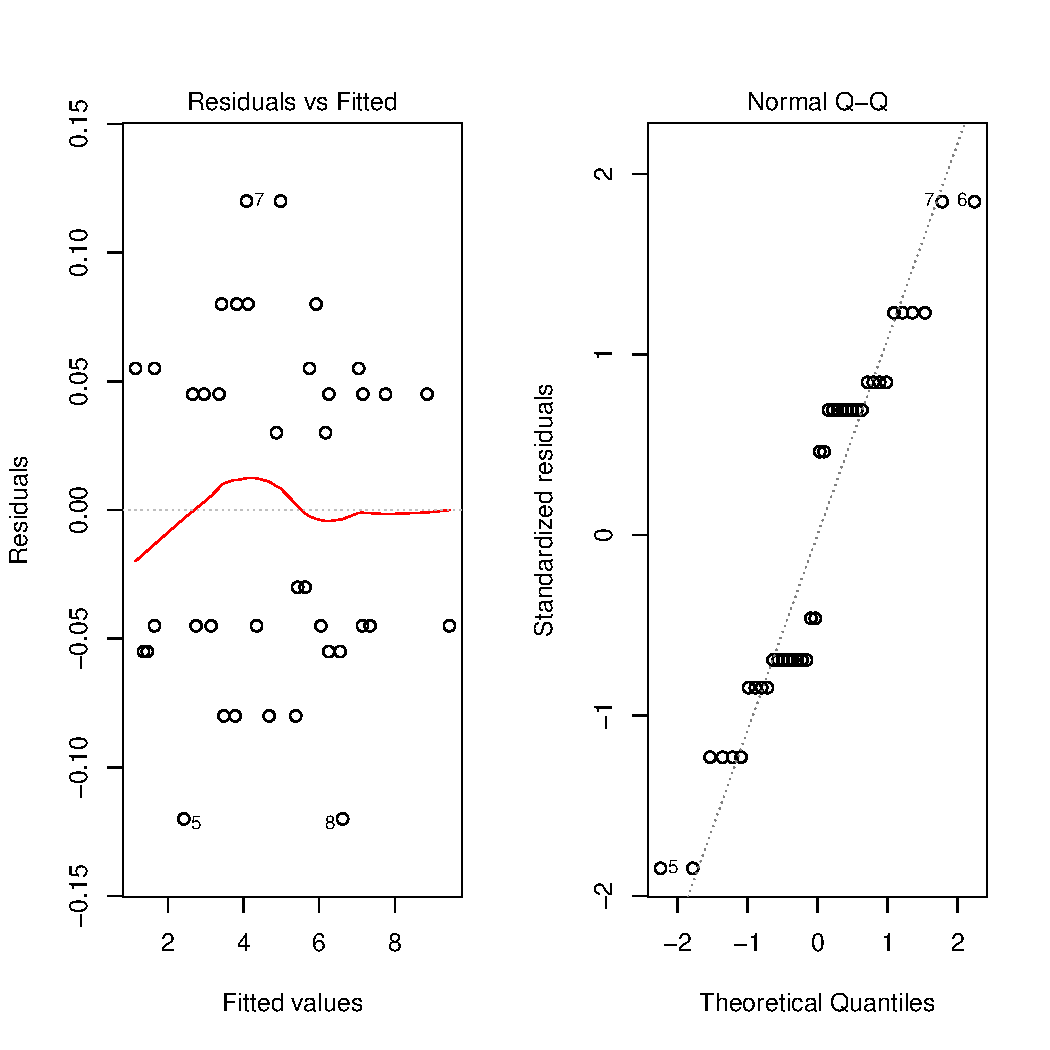
\includegraphics[width=\maxwidth]{figure/unnamed-chunk-8-1} 

\end{knitrout}

\qquad The residuals versus fitted values plots shows no sign for unequal variance.And the QQ-plot indicates approximately normal distribution with slightly light tail, so that normality assumption seems to be reasonable, we can use model here.

\item

\begin{knitrout}
\definecolor{shadecolor}{rgb}{0.969, 0.969, 0.969}\color{fgcolor}\begin{kframe}
\begin{alltt}
  \hlkwd{stripchart}\hlstd{(dat}\hlopt{$}\hlstd{Y} \hlopt{~} \hlstd{dat}\hlopt{$}\hlstd{A}\hlopt{*}\hlstd{dat}\hlopt{$}\hlstd{B,} \hlkwc{method}\hlstd{=}\hlstr{"stack"}\hlstd{)}
\end{alltt}
\end{kframe}
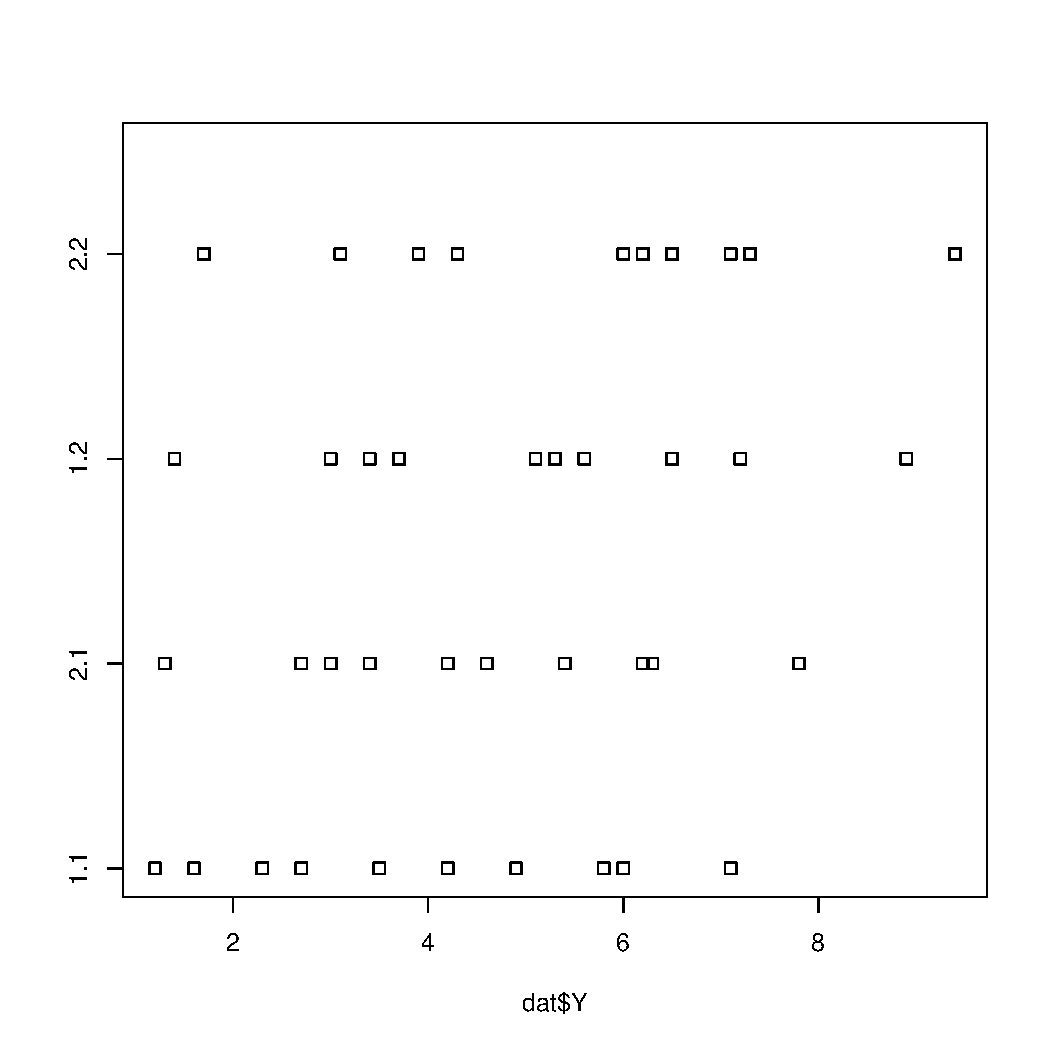
\includegraphics[width=\maxwidth]{figure/unnamed-chunk-9-1} 

\end{knitrout}

\qquad These plots do not indicate any correlations of the error terms within AB, and thus suggest that no interference effects are present.

\end{enumerate}

\section{27.19}

\begin{enumerate}[(a)]

\item

\begin{knitrout}
\definecolor{shadecolor}{rgb}{0.969, 0.969, 0.969}\color{fgcolor}\begin{kframe}
\begin{alltt}
  \hlstd{model} \hlkwb{=} \hlkwd{aov}\hlstd{(Y}\hlopt{~} \hlstd{A}\hlopt{*}\hlstd{B}\hlopt{+}\hlstd{A}\hlopt{*}\hlstd{S}\hlopt{+}\hlstd{B}\hlopt{*}\hlstd{S}\hlopt{+} \hlkwd{Error}\hlstd{(S}\hlopt{/}\hlstd{(A}\hlopt{*}\hlstd{B)),} \hlkwc{data} \hlstd{= dat)}
  \hlkwd{summary}\hlstd{(model)}
\end{alltt}
\begin{verbatim}
## 
## Error: S
##   Df Sum Sq Mean Sq
## S  9  154.6   17.18
## 
## Error: S:A
##     Df Sum Sq Mean Sq
## A    1  3.025  3.0250
## A:S  9  2.035  0.2261
## 
## Error: S:B
##     Df Sum Sq Mean Sq
## B    1 11.449  11.449
## B:S  9  5.061   0.562
## 
## Error: S:A:B
##           Df Sum Sq Mean Sq F value Pr(>F)
## A:B        1  0.001 0.00100   0.053  0.823
## Residuals  9  0.169 0.01878
\end{verbatim}
\end{kframe}
\end{knitrout}

\item

\begin{knitrout}
\definecolor{shadecolor}{rgb}{0.969, 0.969, 0.969}\color{fgcolor}\begin{kframe}
\begin{alltt}
  \hlkwd{interaction.plot}\hlstd{(dat}\hlopt{$}\hlstd{A, dat}\hlopt{$}\hlstd{B, dat}\hlopt{$}\hlstd{Y,} \hlkwc{ylim} \hlstd{=} \hlkwd{c}\hlstd{(}\hlnum{1}\hlstd{,} \hlnum{8}\hlstd{))}
  \hlstd{dat1} \hlkwb{=} \hlstd{dat[} \hlkwd{which}\hlstd{(dat}\hlopt{$}\hlstd{B} \hlopt{==} \hlnum{1}\hlstd{), ]}
  \hlstd{dat2} \hlkwb{=} \hlstd{dat[} \hlkwd{which}\hlstd{(dat}\hlopt{$}\hlstd{B} \hlopt{==} \hlnum{2}\hlstd{), ]}
  \hlkwd{points}\hlstd{(dat1}\hlopt{$}\hlstd{A, dat1}\hlopt{$}\hlstd{Y,} \hlkwc{pch} \hlstd{=} \hlnum{1}\hlstd{)}
  \hlkwd{points}\hlstd{(dat2}\hlopt{$}\hlstd{A, dat2}\hlopt{$}\hlstd{Y,} \hlkwc{pch} \hlstd{=} \hlnum{2}\hlstd{)}
\end{alltt}
\end{kframe}
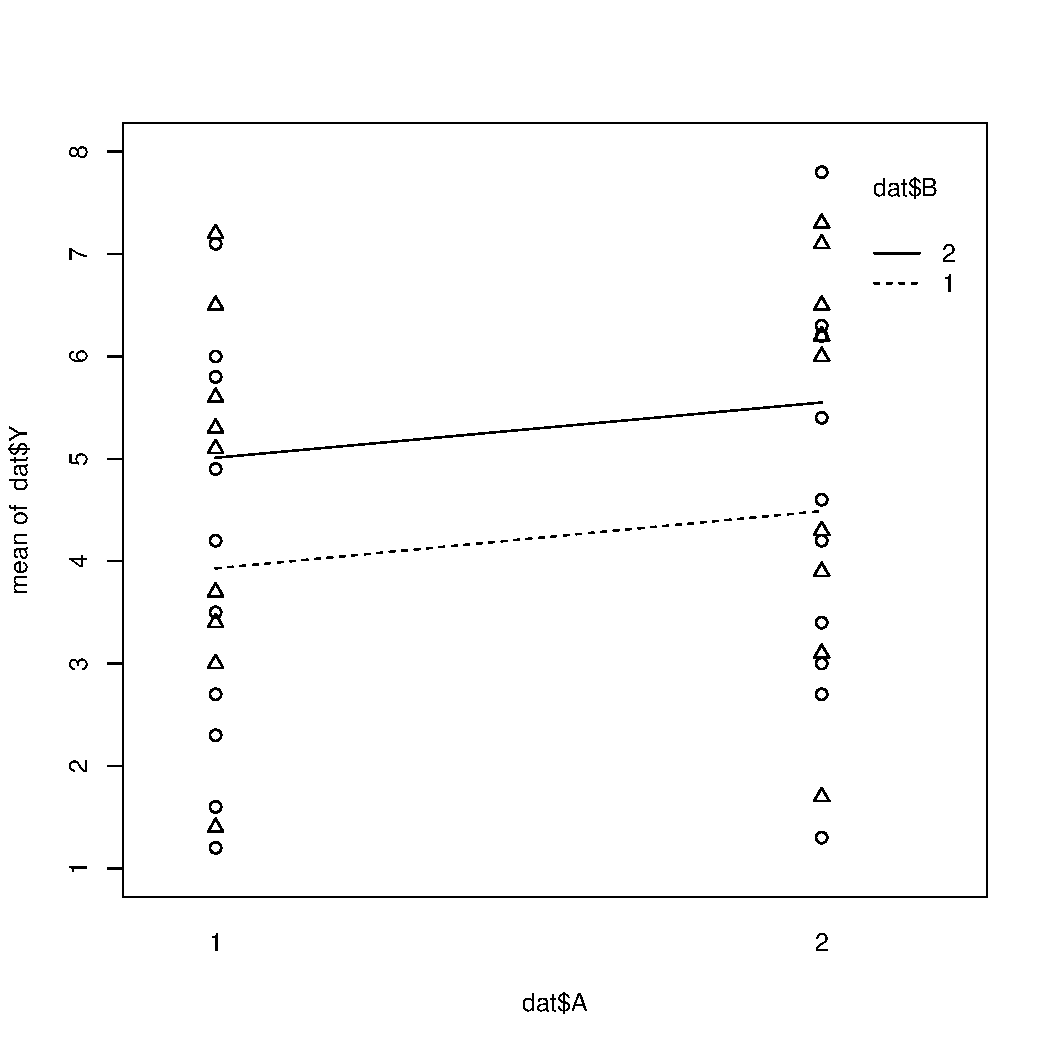
\includegraphics[width=\maxwidth]{figure/unnamed-chunk-11-1} 

\end{knitrout}

\qquad From the plot, we know that treatment interaction effects are not present, but two treatment main effects are present.

\item

\begin{knitrout}
\definecolor{shadecolor}{rgb}{0.969, 0.969, 0.969}\color{fgcolor}\begin{kframe}
\begin{alltt}
  \hlkwd{qf}\hlstd{(}\hlnum{1}\hlopt{-}\hlnum{0.005}\hlstd{,} \hlnum{1}\hlstd{,} \hlnum{9}\hlstd{)}
\end{alltt}
\begin{verbatim}
## [1] 13.61361
\end{verbatim}
\begin{alltt}
  \hlkwd{pf}\hlstd{(}\hlnum{0.053}\hlstd{,} \hlnum{1}\hlstd{,} \hlnum{9}\hlstd{,} \hlkwc{lower.tail} \hlstd{=} \hlnum{FALSE}\hlstd{)}
\end{alltt}
\begin{verbatim}
## [1] 0.8230705
\end{verbatim}
\end{kframe}
\end{knitrout}

\begin{center}
$H_0$:all $(\alpha\beta)_{jk}$ equal zero

VS. $H_1$:not all $(\alpha\beta)_{jk}$ equal zero

$F^*=\frac{MSAB}{MSABS} = 0.001/0.01878  = 0.053$

we can reject $H_0$ if $F^* > F(1-0.005;1,9)=13.61361$,otherwise reject$H_1$

so that reject $H_1$ because $F^*<13.61361$,

therefore, there's no two treatment interaction effect, and the P-value is 0.823
\end{center}

\item

\begin{knitrout}
\definecolor{shadecolor}{rgb}{0.969, 0.969, 0.969}\color{fgcolor}\begin{kframe}
\begin{alltt}
  \hlkwd{qf}\hlstd{(}\hlnum{1}\hlopt{-}\hlnum{0.05}\hlstd{,} \hlnum{1}\hlstd{,} \hlnum{9}\hlstd{)}
\end{alltt}
\begin{verbatim}
## [1] 5.117355
\end{verbatim}
\begin{alltt}
  \hlkwd{pf}\hlstd{(}\hlnum{13.37904}\hlstd{,} \hlnum{1}\hlstd{,} \hlnum{9}\hlstd{,} \hlkwc{lower.tail} \hlstd{=} \hlnum{FALSE}\hlstd{)}
\end{alltt}
\begin{verbatim}
## [1] 0.005253961
\end{verbatim}
\end{kframe}
\end{knitrout}

\begin{center}
$H_0$: all $\alpha_i$ equal zero(i=1,2)

VS. $H_1$:not all $\alpha_i$ equal zero

$F^*=\frac{MSA}{MSAS} = 3.0250/0.2261  = 13.37904$

we can reject $H_0$ if $F^* > F(1-0.05;1,9)=5.117355$,otherwise reject$H_1$

so that reject $H_0$ because $F^*>5.117355$,

therefore, factor A main effect is present, and the P-value is 0.005253961
\end{center}

\begin{knitrout}
\definecolor{shadecolor}{rgb}{0.969, 0.969, 0.969}\color{fgcolor}\begin{kframe}
\begin{alltt}
  \hlkwd{qf}\hlstd{(}\hlnum{1}\hlopt{-}\hlnum{0.05}\hlstd{,} \hlnum{1}\hlstd{,} \hlnum{9}\hlstd{)}
\end{alltt}
\begin{verbatim}
## [1] 5.117355
\end{verbatim}
\begin{alltt}
  \hlkwd{pf}\hlstd{(}\hlnum{20.37189}\hlstd{,} \hlnum{1}\hlstd{,} \hlnum{9}\hlstd{,} \hlkwc{lower.tail} \hlstd{=} \hlnum{FALSE}\hlstd{)}
\end{alltt}
\begin{verbatim}
## [1] 0.001460304
\end{verbatim}
\end{kframe}
\end{knitrout}

\begin{center}
$H_0$: all $\beta_j$ equal zero(j=1,2)

VS. $H_1$:not all $\beta_j$ equal zero

$F^*=\frac{MSB}{MSBS} = 11.449/0.562  = 20.37189$

we can reject $H_0$ if $F^* > F(1-0.05;1,9)=5.117355$,otherwise reject$H_1$

so that reject $H_0$ because $F^*>5.117355$,

therefore, factor B main effect is present, and the P-value is 0.001460304
\end{center}

\item

\begin{knitrout}
\definecolor{shadecolor}{rgb}{0.969, 0.969, 0.969}\color{fgcolor}\begin{kframe}
\begin{alltt}
  \hlstd{means} \hlkwb{=} \hlkwd{with}\hlstd{(dat,} \hlkwd{by}\hlstd{(Y,} \hlkwd{list}\hlstd{(A,B) , mean))}
  \hlstd{L1} \hlkwb{=} \hlstd{means[}\hlnum{2}\hlstd{,}\hlnum{1}\hlstd{]} \hlopt{-} \hlstd{means[}\hlnum{1}\hlstd{,}\hlnum{1}\hlstd{]}
  \hlstd{L2} \hlkwb{=} \hlstd{means[}\hlnum{1}\hlstd{,}\hlnum{2}\hlstd{]} \hlopt{-} \hlstd{means[}\hlnum{1}\hlstd{,}\hlnum{1}\hlstd{]}
  \hlstd{L3} \hlkwb{=} \hlstd{means[}\hlnum{2}\hlstd{,}\hlnum{1}\hlstd{]} \hlopt{-} \hlstd{means[}\hlnum{1}\hlstd{,}\hlnum{2}\hlstd{]}
  \hlstd{L4} \hlkwb{=} \hlstd{means[}\hlnum{2}\hlstd{,}\hlnum{2}\hlstd{]} \hlopt{-} \hlstd{means[}\hlnum{1}\hlstd{,}\hlnum{1}\hlstd{]}
  \hlstd{B} \hlkwb{=} \hlkwd{qt}\hlstd{(}\hlnum{1}\hlopt{-}\hlnum{0.05}\hlopt{/}\hlstd{(}\hlnum{2}\hlopt{*}\hlnum{4}\hlstd{),} \hlnum{9}\hlstd{)}
  \hlstd{B}
\end{alltt}
\begin{verbatim}
## [1] 3.110935
\end{verbatim}
\begin{alltt}
  \hlstd{msabs} \hlkwb{=} \hlnum{0.01878}
  \hlstd{S} \hlkwb{=} \hlkwd{sqrt}\hlstd{(}\hlnum{2}\hlopt{*}\hlstd{msabs}\hlopt{/}\hlstd{(s))}
  \hlstd{S}
\end{alltt}
\begin{verbatim}
## [1] 0.06128621
\end{verbatim}
\begin{alltt}
  \hlkwd{c}\hlstd{(L1}\hlopt{-}\hlstd{S}\hlopt{*}\hlstd{B, L1}\hlopt{+}\hlstd{S}\hlopt{*}\hlstd{B)}
\end{alltt}
\begin{verbatim}
## [1] 0.3693426 0.7506574
\end{verbatim}
\begin{alltt}
  \hlkwd{c}\hlstd{(L2}\hlopt{-}\hlstd{S}\hlopt{*}\hlstd{B, L2}\hlopt{+}\hlstd{S}\hlopt{*}\hlstd{B)}
\end{alltt}
\begin{verbatim}
## [1] 0.8893426 1.2706574
\end{verbatim}
\begin{alltt}
  \hlkwd{c}\hlstd{(L3}\hlopt{-}\hlstd{S}\hlopt{*}\hlstd{B, L3}\hlopt{+}\hlstd{S}\hlopt{*}\hlstd{B)}
\end{alltt}
\begin{verbatim}
## [1] -0.7106574 -0.3293426
\end{verbatim}
\begin{alltt}
  \hlkwd{c}\hlstd{(L4}\hlopt{-}\hlstd{S}\hlopt{*}\hlstd{B, L4}\hlopt{+}\hlstd{S}\hlopt{*}\hlstd{B)}
\end{alltt}
\begin{verbatim}
## [1] 1.429343 1.810657
\end{verbatim}
\end{kframe}
\end{knitrout}

\begin{displaymath}
\begin{split}
\bar{Y}_{\cdot 11} =3.936 &, \bar{Y}_{\cdot 12} = 5.01 ,\\
\bar{Y}_{\cdot 21} =4.49 &, \bar{Y}_{\cdot 22} = 5.55 \\
\hat{L}_1 = \bar{Y}_{\cdot 21}-\bar{Y}_{\cdot 11} = .56 &,  
\hat{L}_2 = \bar{Y}_{\cdot 12}-\bar{Y}_{\cdot 21}= 1.08 ,\\ 
\hat{L}_3 = \bar{Y}_{\cdot 21}-\bar{Y}_{\cdot 12}=-.52 &,
\hat{L}_4 = \bar{Y}_{\cdot 22}-\bar{Y}_{\cdot 11} =1.62 \\
S = \sqrt{\frac{MSABS}{s}*2} = 0.06128621 &, B = t(1-\alpha/(2*4), (a-1)(b-1)(s-1))=3.110935\\
\text{base on} &\hat{L}_i \pm S*B\\
0.3693426 & \leq L_1 \leq 0.7506574  \\
0.8893426 &\leq L_2 \leq 1.2706574\\
-0.7106574 &\leq L_3 \leq -0.3293426 \\
1.429343 & \leq L_4 \leq 1.810657 \\
\end{split}
\end{displaymath}

\qquad The treatment of high dose of both drugs has the most significant reduction in pain intensity compared to the treatments of only one drug has high dose , and a significant difference exists in the mean effects of two drugs used alone.

\end{enumerate}

\section{27.20}

\begin{enumerate}[(a)]

\item

\begin{knitrout}
\definecolor{shadecolor}{rgb}{0.969, 0.969, 0.969}\color{fgcolor}\begin{kframe}
\begin{alltt}
  \hlstd{dat} \hlkwb{=} \hlkwd{read.table}\hlstd{(}\hlstr{"CH27PR20.txt"}\hlstd{)}
  \hlkwd{names}\hlstd{(dat)} \hlkwb{=} \hlkwd{c}\hlstd{(}\hlstr{"Y"}\hlstd{,} \hlstr{"S"}\hlstd{,} \hlstr{"A"}\hlstd{,} \hlstr{"B"}\hlstd{)}
  \hlstd{dat}\hlopt{$}\hlstd{S} \hlkwb{=} \hlkwd{factor}\hlstd{(dat}\hlopt{$}\hlstd{S)}
  \hlstd{dat}\hlopt{$}\hlstd{A} \hlkwb{=} \hlkwd{factor}\hlstd{(dat}\hlopt{$}\hlstd{A)}
  \hlstd{dat}\hlopt{$}\hlstd{B} \hlkwb{=} \hlkwd{factor}\hlstd{(dat}\hlopt{$}\hlstd{B)}
  \hlstd{s} \hlkwb{=} \hlkwd{length}\hlstd{(}\hlkwd{unique}\hlstd{(dat}\hlopt{$}\hlstd{S))}
  \hlstd{a} \hlkwb{=} \hlkwd{length}\hlstd{(}\hlkwd{unique}\hlstd{(dat}\hlopt{$}\hlstd{A))}
  \hlstd{b} \hlkwb{=} \hlkwd{length}\hlstd{(}\hlkwd{unique}\hlstd{(dat}\hlopt{$}\hlstd{B))}
  \hlstd{model} \hlkwb{=} \hlkwd{aov}\hlstd{(Y}\hlopt{~} \hlstd{A}\hlopt{*}\hlstd{B}\hlopt{+}\hlstd{(A}\hlopt{/}\hlstd{S),} \hlkwc{data} \hlstd{= dat)}
  \hlkwd{resid}\hlstd{(model)}
\end{alltt}
\begin{verbatim}
##    1    2    3    4    5    6    7    8    9   10   11   12   13   14   15 
## -0.6  0.6 -1.7  1.7  0.4 -0.4  1.3 -1.3 -0.6  0.6  0.3 -0.3  0.4 -0.4 -0.2 
##   16   17   18   19   20 
##  0.2  0.4 -0.4  0.3 -0.3
\end{verbatim}
\begin{alltt}
  \hlkwd{par}\hlstd{(}\hlkwc{mfrow} \hlstd{=} \hlkwd{c}\hlstd{(}\hlnum{1}\hlstd{,}\hlnum{2}\hlstd{))}
  \hlkwd{plot}\hlstd{(model,} \hlkwc{which} \hlstd{=} \hlnum{1}\hlstd{)}
  \hlkwd{plot}\hlstd{(model,} \hlkwc{which} \hlstd{=} \hlnum{2}\hlstd{)}
\end{alltt}
\end{kframe}
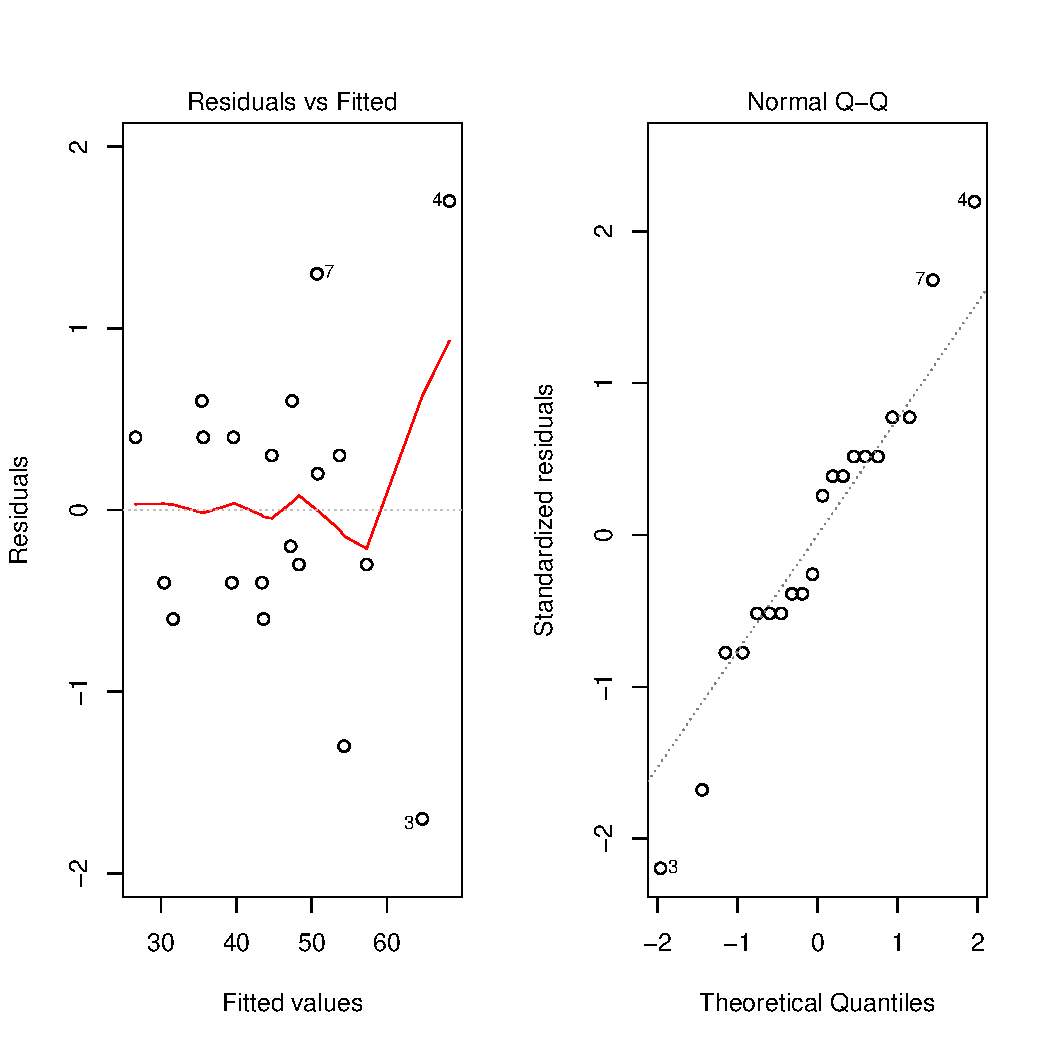
\includegraphics[width=\maxwidth]{figure/unnamed-chunk-16-1} 

\end{knitrout}

\qquad The residuals versus fitted values plots shows no sign for unequal variance.And the QQ-plot indicates approximately normal distribution with slightly heavy tail, so that normality assumption seems to be reasonable, we can use model here.

\item

\begin{knitrout}
\definecolor{shadecolor}{rgb}{0.969, 0.969, 0.969}\color{fgcolor}\begin{kframe}
\begin{alltt}
  \hlstd{dat1} \hlkwb{=} \hlstd{dat[} \hlkwd{which}\hlstd{(dat}\hlopt{$}\hlstd{A} \hlopt{==} \hlnum{1}\hlstd{), ]}
  \hlstd{dat2} \hlkwb{=} \hlstd{dat[} \hlkwd{which}\hlstd{(dat}\hlopt{$}\hlstd{A} \hlopt{==} \hlnum{2}\hlstd{), ]}
  \hlkwd{par}\hlstd{(} \hlkwc{mfrow} \hlstd{=} \hlkwd{c}\hlstd{(}\hlnum{1}\hlstd{,} \hlnum{2}\hlstd{))}
  \hlkwd{interaction.plot}\hlstd{(dat1}\hlopt{$}\hlstd{B, dat1}\hlopt{$}\hlstd{S, dat1}\hlopt{$}\hlstd{Y)}
  \hlkwd{interaction.plot}\hlstd{(dat2}\hlopt{$}\hlstd{B, dat2}\hlopt{$}\hlstd{S, dat2}\hlopt{$}\hlstd{Y)}
\end{alltt}
\end{kframe}
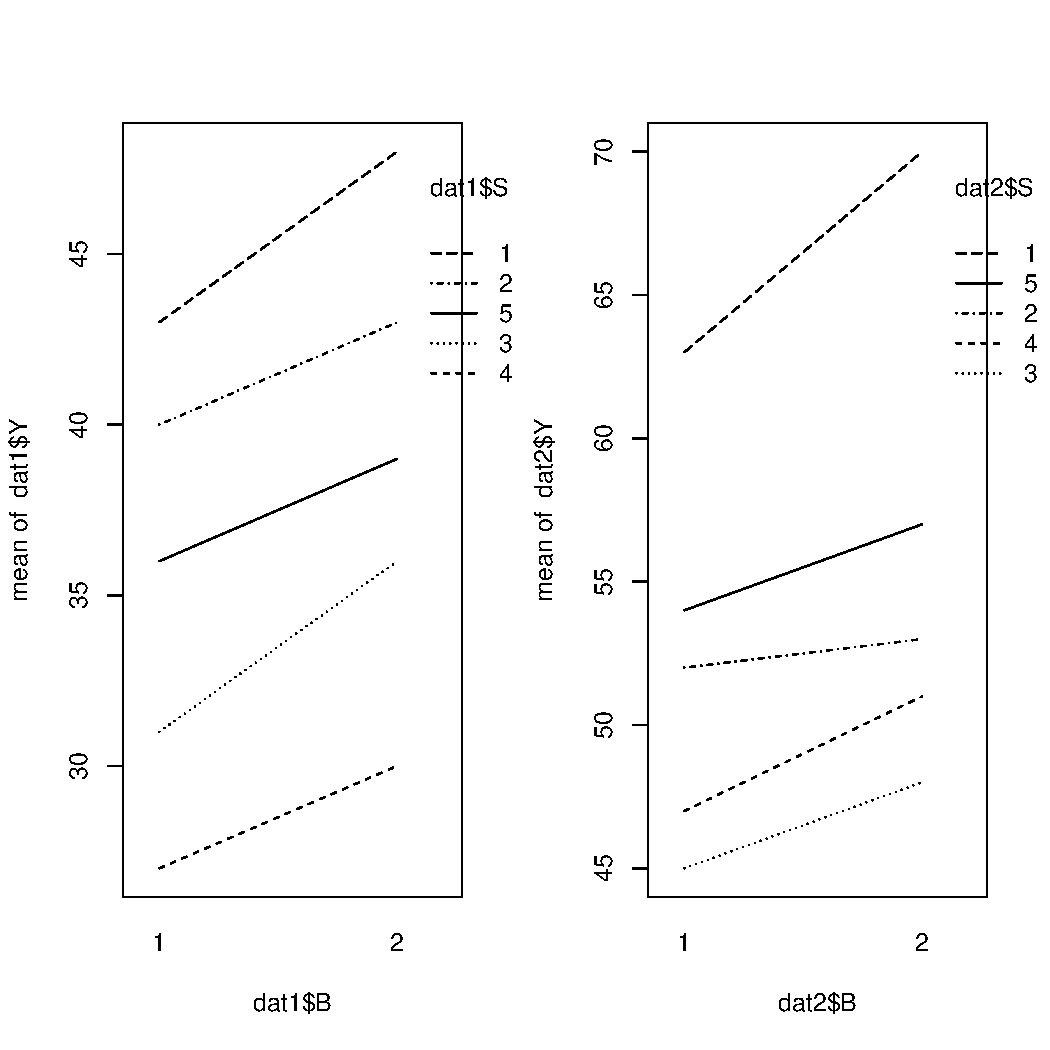
\includegraphics[width=\maxwidth]{figure/unnamed-chunk-17-1} 

\end{knitrout}

\qquad There's no evidence any interactions between field and treatments, so split-plot design can be used here.

\end{enumerate}

\section{27.21}

\begin{enumerate}[(a)]

\item

\begin{knitrout}
\definecolor{shadecolor}{rgb}{0.969, 0.969, 0.969}\color{fgcolor}\begin{kframe}
\begin{alltt}
  \hlstd{model} \hlkwb{=} \hlkwd{aov}\hlstd{(Y}\hlopt{~} \hlstd{A}\hlopt{*}\hlstd{B}\hlopt{+}\hlkwd{Error}\hlstd{(A}\hlopt{/}\hlstd{S),} \hlkwc{data} \hlstd{= dat)}
  \hlkwd{summary}\hlstd{(model)}
\end{alltt}
\begin{verbatim}
## 
## Error: A
##   Df Sum Sq Mean Sq
## A  1   1394    1394
## 
## Error: A:S
##           Df Sum Sq Mean Sq F value Pr(>F)
## Residuals  8  837.6   104.7               
## 
## Error: Within
##           Df Sum Sq Mean Sq F value   Pr(>F)    
## B          1  68.45   68.45  45.633 0.000144 ***
## A:B        1   0.05    0.05   0.033 0.859674    
## Residuals  8  12.00    1.50                     
## ---
## Signif. codes:  0 '***' 0.001 '**' 0.01 '*' 0.05 '.' 0.1 ' ' 1
\end{verbatim}
\end{kframe}
\end{knitrout}

\item

\begin{knitrout}
\definecolor{shadecolor}{rgb}{0.969, 0.969, 0.969}\color{fgcolor}\begin{kframe}
\begin{alltt}
  \hlkwd{interaction.plot}\hlstd{(dat}\hlopt{$}\hlstd{A, dat}\hlopt{$}\hlstd{B, dat}\hlopt{$}\hlstd{Y,} \hlkwc{ylim} \hlstd{=} \hlkwd{c}\hlstd{(}\hlnum{25}\hlstd{,} \hlnum{75}\hlstd{))}
  \hlstd{dat1} \hlkwb{=} \hlstd{dat[} \hlkwd{which}\hlstd{(dat}\hlopt{$}\hlstd{B} \hlopt{==} \hlnum{1}\hlstd{), ]}
  \hlstd{dat2} \hlkwb{=} \hlstd{dat[} \hlkwd{which}\hlstd{(dat}\hlopt{$}\hlstd{B} \hlopt{==} \hlnum{2}\hlstd{), ]}
  \hlkwd{points}\hlstd{(dat1}\hlopt{$}\hlstd{A, dat1}\hlopt{$}\hlstd{Y,} \hlkwc{pch} \hlstd{=} \hlnum{1}\hlstd{)}
  \hlkwd{points}\hlstd{(dat2}\hlopt{$}\hlstd{A, dat2}\hlopt{$}\hlstd{Y,} \hlkwc{pch} \hlstd{=} \hlnum{2}\hlstd{)}
\end{alltt}
\end{kframe}
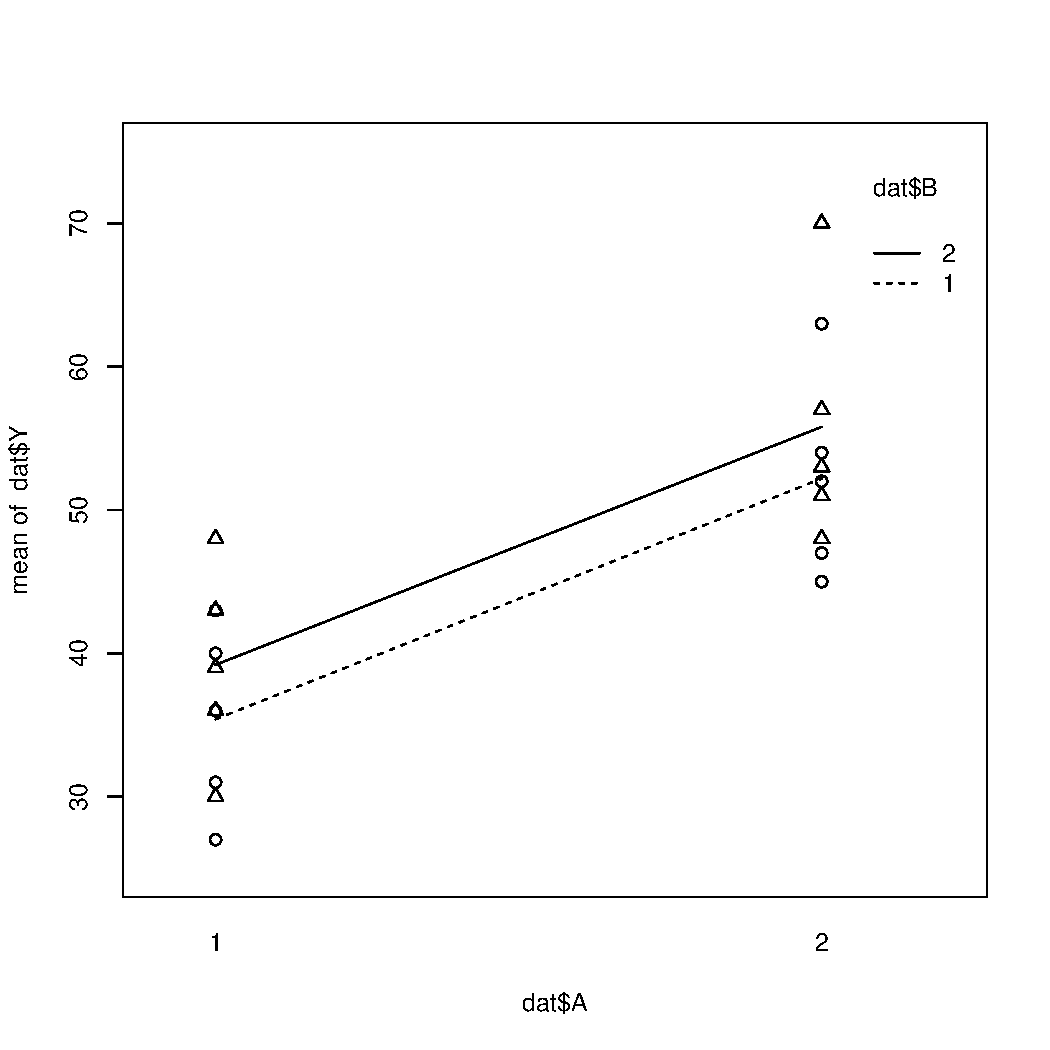
\includegraphics[width=\maxwidth]{figure/unnamed-chunk-19-1} 

\end{knitrout}

\qquad From the plot, we know that treatment interaction effects are not present, but two treatment main effects are present.

\item

\begin{knitrout}
\definecolor{shadecolor}{rgb}{0.969, 0.969, 0.969}\color{fgcolor}\begin{kframe}
\begin{alltt}
  \hlkwd{qf}\hlstd{(}\hlnum{1}\hlopt{-}\hlnum{0.05}\hlstd{,} \hlnum{1}\hlstd{,} \hlnum{8}\hlstd{)}
\end{alltt}
\begin{verbatim}
## [1] 5.317655
\end{verbatim}
\begin{alltt}
  \hlkwd{pf}\hlstd{(}\hlnum{0.033}\hlstd{,} \hlnum{1}\hlstd{,} \hlnum{8}\hlstd{,} \hlkwc{lower.tail} \hlstd{=} \hlnum{FALSE}\hlstd{)}
\end{alltt}
\begin{verbatim}
## [1] 0.8603687
\end{verbatim}
\end{kframe}
\end{knitrout}

\begin{center}
$H_0$:all $(\alpha\beta)_{jk}$ equal zero

VS. $H_1$:not all $(\alpha\beta)_{jk}$ equal zero

$F^*=\frac{MSAB}{MSB.W(A)} = 0.05/1.5  = 0.033$

we can reject $H_0$ if $F^* > F(1-0.05; 1, 8)=5.317655$,otherwise reject$H_1$

so that reject $H_1$ because $F^*<5.317655$,

therefore, there's no two treatment interaction effect, and the P-value is 0.8603687
\end{center}

\item

\begin{knitrout}
\definecolor{shadecolor}{rgb}{0.969, 0.969, 0.969}\color{fgcolor}\begin{kframe}
\begin{alltt}
  \hlkwd{qf}\hlstd{(}\hlnum{1}\hlopt{-}\hlnum{0.05}\hlstd{,} \hlnum{1}\hlstd{,} \hlnum{8}\hlstd{)}
\end{alltt}
\begin{verbatim}
## [1] 5.317655
\end{verbatim}
\begin{alltt}
  \hlkwd{pf}\hlstd{(}\hlnum{13.31423}\hlstd{,} \hlnum{1}\hlstd{,} \hlnum{8}\hlstd{,} \hlkwc{lower.tail} \hlstd{=} \hlnum{FALSE}\hlstd{)}
\end{alltt}
\begin{verbatim}
## [1] 0.006505011
\end{verbatim}
\end{kframe}
\end{knitrout}

\begin{center}
$H_0$: all $\alpha_i$ equal zero(i=1,2)

VS. $H_1$:not all $\alpha_i$ equal zero

$F^*=\frac{MSA}{MSW(A)} = 1394/104.7  = 13.31423$

we can reject $H_0$ if $F^* > F(1-0.05;1,8)=5.317655$,otherwise reject$H_1$

so that reject $H_0$ because $F^*>5.317655$,

therefore, factor A effect is present, and the P-value is 0.00650501
\end{center}

\begin{knitrout}
\definecolor{shadecolor}{rgb}{0.969, 0.969, 0.969}\color{fgcolor}\begin{kframe}
\begin{alltt}
  \hlkwd{qf}\hlstd{(}\hlnum{1}\hlopt{-}\hlnum{0.05}\hlstd{,} \hlnum{1}\hlstd{,} \hlnum{8}\hlstd{)}
\end{alltt}
\begin{verbatim}
## [1] 5.317655
\end{verbatim}
\begin{alltt}
  \hlkwd{pf}\hlstd{(}\hlnum{45.63333}\hlstd{,} \hlnum{1}\hlstd{,} \hlnum{8}\hlstd{,} \hlkwc{lower.tail} \hlstd{=} \hlnum{FALSE}\hlstd{)}
\end{alltt}
\begin{verbatim}
## [1] 0.0001442759
\end{verbatim}
\end{kframe}
\end{knitrout}

\begin{center}
$H_0$: all $\beta_j$ equal zero(j=1,2)

VS. $H_1$:not all $\beta_j$ equal zero

$F^*=\frac{MSB}{MSB.W(A)} = 68.45/1.5  = 45.63333$

we can reject $H_0$ if $F^* > F(1-0.05;1,8)=5.317655$,otherwise reject$H_1$

so that reject $H_0$ because $F^*>5.317655$,

therefore, factor B main effect is present, and the P-value is 0.0001442759
\end{center}

\item

\begin{knitrout}
\definecolor{shadecolor}{rgb}{0.969, 0.969, 0.969}\color{fgcolor}\begin{kframe}
\begin{alltt}
  \hlstd{means1} \hlkwb{=} \hlkwd{with}\hlstd{(dat,} \hlkwd{by}\hlstd{(Y, A , mean))}
  \hlstd{means2} \hlkwb{=} \hlkwd{with}\hlstd{(dat,} \hlkwd{by}\hlstd{(Y, B , mean))}
  \hlstd{L1} \hlkwb{=} \hlstd{means1[}\hlnum{1}\hlstd{]} \hlopt{-} \hlstd{means1[}\hlnum{2}\hlstd{]}
  \hlstd{L2} \hlkwb{=} \hlstd{means2[}\hlnum{1}\hlstd{]} \hlopt{-} \hlstd{means2[}\hlnum{2}\hlstd{]}
  \hlstd{B} \hlkwb{=} \hlkwd{qt}\hlstd{(}\hlnum{1}\hlopt{-}\hlnum{0.1}\hlopt{/}\hlstd{(}\hlnum{2}\hlopt{*}\hlnum{2}\hlstd{),} \hlnum{8}\hlstd{)}
  \hlstd{B}
\end{alltt}
\begin{verbatim}
## [1] 2.306004
\end{verbatim}
\begin{alltt}
  \hlstd{msb.wa} \hlkwb{=} \hlnum{1.5}
  \hlstd{mswa} \hlkwb{=} \hlnum{104.7}
  \hlstd{S1} \hlkwb{=} \hlkwd{sqrt}\hlstd{(}\hlnum{2}\hlopt{*}\hlstd{mswa}\hlopt{/}\hlstd{(b}\hlopt{*}\hlstd{s))}
  \hlstd{S2} \hlkwb{=} \hlkwd{sqrt}\hlstd{(}\hlnum{2}\hlopt{*}\hlstd{msb.wa}\hlopt{/}\hlstd{(a}\hlopt{*}\hlstd{s))}
  \hlstd{S1}
\end{alltt}
\begin{verbatim}
## [1] 4.576024
\end{verbatim}
\begin{alltt}
  \hlstd{S2}
\end{alltt}
\begin{verbatim}
## [1] 0.5477226
\end{verbatim}
\begin{alltt}
  \hlkwd{c}\hlstd{(L1}\hlopt{-}\hlstd{S1}\hlopt{*}\hlstd{B, L1}\hlopt{+}\hlstd{S1}\hlopt{*}\hlstd{B)}
\end{alltt}
\begin{verbatim}
##          1          1 
## -27.252331  -6.147669
\end{verbatim}
\begin{alltt}
  \hlkwd{c}\hlstd{(L2}\hlopt{-}\hlstd{S2}\hlopt{*}\hlstd{B, L2}\hlopt{+}\hlstd{S2}\hlopt{*}\hlstd{B)}
\end{alltt}
\begin{verbatim}
##        1        1 
## -4.96305 -2.43695
\end{verbatim}
\end{kframe}
\end{knitrout}

\begin{displaymath}
\begin{split}
\bar{Y}_{\cdot 1 \cdot} =37.3&, \bar{Y}_{\cdot 2 \cdot} = 54 ,\\
\bar{Y}_{\cdot \cdot 1} =43.8 &, \bar{Y}_{\cdot \cdot 2} = 47.5 \\
\hat{L}_1 = \bar{Y}_{\cdot 1 \cdot}-\bar{Y}_{\cdot 2 \cdot}  = -16.7 &,  
\hat{L}_2 = \bar{Y}_{\cdot \cdot 1}-\bar{Y}_{\cdot \cdot 2} =-3.7\\ 
B = t(1-\alpha/(2*2), a(b-1)(s-1)) &=2.306004\\
S1 = \sqrt{\frac{MSW(A)}{bs}*2} = 4.576024 &,
S2 = \sqrt{\frac{MSB.W(A)}{as}*2} = 0.5477226 \\
\text{base on} &\hat{L}_i \pm S*B\\
-27.252331 & \leq L_1 \leq -6.147669  \\
-4.96305 &\leq L_2 \leq -2.43695 \\
\end{split}
\end{displaymath}

\qquad Irrigation method 2 is significantly better than Irrigation method 1, and fertilizer 2 is significantly better than fertilizer 1.

\end{enumerate}

\section{27.22}

\begin{displaymath}
\begin{split}
SSTO &= \sum_i \sum_j (Y_{ij}-\bar{Y}_{\cdot \cdot})^2 \\
     &= \sum_i \sum_j (Y_{ij} -\bar{Y}_{i\cdot} + \bar{Y}_{i\cdot} -\bar{Y}_{\cdot \cdot})^2 \\
     &= \sum_i \sum_j (Y_{ij} -\bar{Y}_{i\cdot})^2 + \sum_i \sum_j (\bar{Y}_{i\cdot} -\bar{Y}_{\cdot \cdot})^2 + 2\sum_i \sum_j(Y_{ij} -\bar{Y}_{i\cdot})(\bar{Y}_{i\cdot}-\bar{Y}_{\cdot \cdot})\\
     &= \sum_i \sum_j (Y_{ij} -\bar{Y}_{i\cdot})^2 + \sum_i \sum_j (\bar{Y}_{i\cdot} -\bar{Y}_{\cdot \cdot})^2 + 2\sum_i [(\bar{Y}_{i\cdot}-\bar{Y}_{\cdot \cdot})*\sum_j (Y_{ij} -\bar{Y}_{i\cdot})]\\
     &\text{(since } \sum_j (Y_{ij} -\bar{Y}_{i\cdot})=0 \text{)}\\
     &= \sum_i \sum_j (Y_{ij} -\bar{Y}_{i\cdot})^2 + r\sum_i (\bar{Y}_{i\cdot} -\bar{Y}_{\cdot \cdot})^2\\
     &= SSS + SSW
\end{split}
\end{displaymath}

\section{Extra Problem}

Base on:

\begin{displaymath}
\begin{split}
Y_{ij} &= \mu_{\cdot\cdot} + \rho_i + \tau_j + \epsilon_{ij}\\
\bar{Y}_{i\cdot} &= \mu_{\cdot\cdot} + \rho_i + \bar{\epsilon}_{i\cdot}\\
\bar{Y}_{\cdot j} &= \mu_{\cdot\cdot} + \bar{\rho}_\cdot + \tau_j + \bar{\epsilon}_{\cdot j}\\
\bar{Y}_{\cdot \cdot} &= \mu_{\cdot\cdot} + \bar{\rho}_\cdot + \bar{\epsilon}_{\cdot \cdot}\\
\end{split}
\end{displaymath}

So that:

\begin{displaymath}
\begin{split}
E(SSS) &= r \sum_i (E(\bar{Y}_{i\cdot}-\bar{Y}_{\cdot\cdot})^2) \\
       &= r \sum_i (Var(\bar{Y}_{i\cdot}-\bar{Y}_{\cdot\cdot})+ [E(\bar{Y}_{i\cdot}-\bar{Y}_{\cdot\cdot})]^2)\\
       &\text{(since } E(\bar{Y}_{i\cdot}-\bar{Y}_{\cdot\cdot})=0 \text{)}\\  
       &= r \sum_i (Var(\bar{Y}_{i\cdot}) + Var(\bar{Y}_{\cdot\cdot}) - 2 Cov((\bar{Y}_{i\cdot}, \bar{Y}_{\cdot\cdot}))\\
       &= r \sum_i ( (\sigma_\rho^2+ \frac{\sigma^2}{r}) + (\frac{\sigma_\rho^2}{s}+ \frac{\sigma^2}{rs}) -2*(Cov(\rho_i,\bar{\rho}_\cdot)+Cov(\bar{\epsilon}_{i\cdot}, \bar{\rho}_\cdot)+Cov(\rho_i, \bar{\epsilon}_{\cdot \cdot})+Cov(\bar{\epsilon}_{i\cdot}, \bar{\epsilon}_{\cdot \cdot}))\\
       &= rs * ( (\sigma_\rho^2+ \frac{\sigma^2}{r}) + (\frac{\sigma_\rho^2}{s}+ \frac{\sigma^2}{rs}) -2*(\frac{\sigma_\rho^2}{s} + 0+ 0 + \frac{\sigma^2}{rs}))\\
       &= (s-1)\sigma^2 + r(s-1)\sigma_\rho^2\\
E(MSS) &= \frac{E(SSS)}{s-1}\\
       &= \sigma^2 + r\sigma_\rho^2
\end{split}
\end{displaymath}

Likewise:

\begin{displaymath}
\begin{split}
E(SSTR) &= s \sum_j (E(\bar{Y}_{\cdot j}-\bar{Y}_{\cdot\cdot})^2) \\
       &= s \sum_j (Var(\bar{Y}_{\cdot j}-\bar{Y}_{\cdot\cdot})+ [E(\bar{Y}_{\cdot j}-\bar{Y}_{\cdot\cdot})]^2)\\ 
       &= s \sum_j (Var(\bar{Y}_{\cdot j}) + Var(\bar{Y}_{\cdot\cdot}) - 2 Cov((\bar{Y}_{\cdot j}, \bar{Y}_{\cdot\cdot}) + \tau_j)\\
       &= s \sum_j ( (\frac{\sigma_\rho^2}{s}+ \frac{\sigma^2}{s}) + (\frac{\sigma_\rho^2}{s}+ \frac{\sigma^2}{rs}) -2*(\frac{\sigma_\rho^2}{s} + 0+ 0 + \frac{\sigma^2}{rs}) + \tau_j)\\
       &= (r-1)\sigma^2 + s\sum \tau_j^2\\
E(MSTR) &= \frac{E(SSTR)}{r-1}\\
       &= \sigma^2 + s\frac{\sum \tau_j^2}{r-1}
\end{split}
\end{displaymath}

\begin{displaymath}
\begin{split}
E(SSTR.S) &= \sum_i \sum_j (E(Y_{ij}-\bar{Y}_{i\cdot}-\bar{Y}_{\cdot j}+\bar{Y}_{\cdot\cdot})^2) \\
       &= \sum_i \sum_j (Var(Y_{ij}-\bar{Y}_{i\cdot}-\bar{Y}_{\cdot j}+\bar{Y}_{\cdot\cdot})+ [E(Y_{ij}-\bar{Y}_{i\cdot}-\bar{Y}_{\cdot j}+\bar{Y}_{\cdot\cdot})]^2)\\ 
       &= \sum_i \sum_j (Var(Y_{ij}-\bar{Y}_{i\cdot}-\bar{Y}_{\cdot j}+\bar{Y}_{\cdot\cdot}))\\
       &= (r-1)(s-1)\sigma^2\\
E(MSTR.S) &= \frac{E(SSTR.S)}{(r-1)(s-1)}\\
       &= \sigma^2
\end{split}
\end{displaymath}

\end{document}
